\documentclass[12pt,a4paper]{article}
\usepackage[margin=1in]{geometry}
\usepackage{amsmath,amssymb}
\usepackage{graphicx}
\usepackage{booktabs}
\usepackage{hyperref}
\usepackage{float}
\usepackage{listings}
\usepackage{xcolor}
\usepackage{subcaption}
\usepackage{multirow}

% Code listing style
\lstset{
    basicstyle=\ttfamily\small,
    breaklines=true,
    frame=single,
    backgroundcolor=\color{gray!10},
    keywordstyle=\color{blue},
    commentstyle=\color{green!50!black},
    stringstyle=\color{red!70!black},
}

\title{
    \textbf{CSL 7640: Natural Language Understanding} \\
    \Large Assignment 2 Report
}
\author{
    Saurav Soni \\
    Roll No: B22AI035 \\
    IIT Jodhpur \\[0.5em]
    \small GitHub: \url{https://github.com/sauravsoni6377/NLU-Assignment-2}
}
\date{\today}

\begin{document}

\maketitle
\tableofcontents
\newpage

% ============================================================
\section{Problem 1: Learning Word Embeddings from IIT Jodhpur Data}
% ============================================================

\subsection{Task 1: Dataset Preparation}

\subsubsection{Data Sources}
Textual data was collected from the IIT Jodhpur official website (\texttt{iitj.ac.in}) using web scraping with Python's \texttt{requests} and \texttt{BeautifulSoup} libraries. Data was gathered from the following sources:

\begin{enumerate}
    \item \textbf{Department and Academic Program Pages:} Information from all departments (CSE, EE, ME, Mathematics, Physics, Chemistry, HSS, etc.), academic programs (B.Tech, M.Tech, M.Sc, Ph.D), and research pages.
    \item \textbf{Academic Regulation Documents (Mandatory):} Academic regulations, examination guidelines, grading system, and academic calendar pages.
    \item \textbf{Faculty Profile Pages:} Faculty listings and individual profile pages across departments.
    \item \textbf{Course Syllabi and Miscellaneous Pages:} Course catalogue, placement statistics, student activities, alumni pages, campus infrastructure, library, and general about pages.
\end{enumerate}

\subsubsection{Preprocessing Pipeline}
The raw text was processed through the following steps:
\begin{enumerate}
    \item \textbf{Boilerplate Removal:} Script, style, navigation, and footer tags were removed. URLs, email addresses, and HTML entities were stripped.
    \item \textbf{Non-English Text Removal:} Non-ASCII characters (Hindi and other language text) were removed using regex filtering.
    \item \textbf{Tokenization:} NLTK's \texttt{word\_tokenize} was used for robust tokenization that handles contractions and abbreviations.
    \item \textbf{Lowercasing:} All tokens were converted to lowercase for normalization.
    \item \textbf{Filtering:} Stopwords (NLTK English stopwords), web boilerplate words, tokens shorter than 2 characters, and purely numeric/punctuation tokens were removed.
\end{enumerate}

\subsubsection{Dataset Statistics}

\begin{table}[H]
\centering
\caption{Corpus Statistics}
\begin{tabular}{lr}
\toprule
\textbf{Metric} & \textbf{Value} \\
\midrule
Total Documents & 100 \\
Total Tokens (after preprocessing) & 33,454 \\
Vocabulary Size (unique tokens) & 3,847 \\
Average Tokens per Document & 334.5 \\
\bottomrule
\end{tabular}
\end{table}

\subsubsection{Word Cloud}

\begin{figure}[H]
\centering
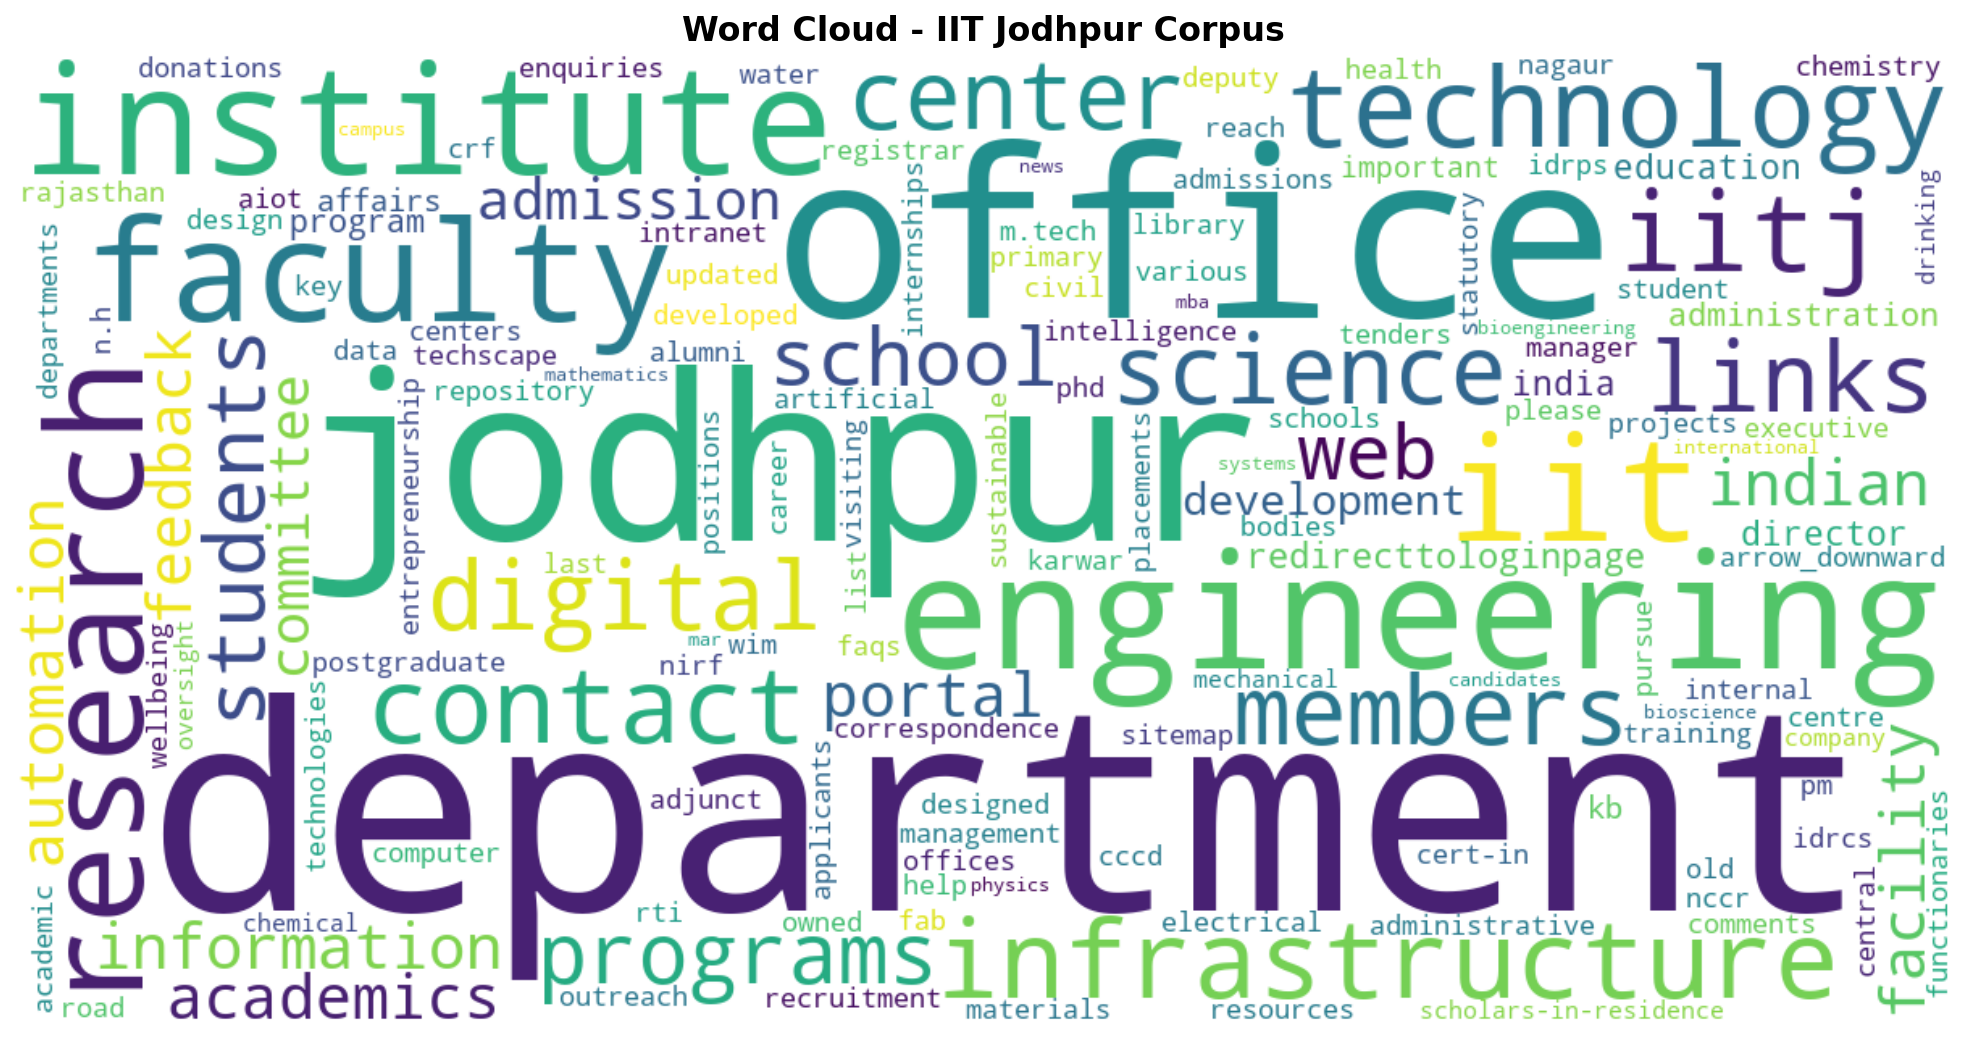
\includegraphics[width=0.85\textwidth]{../problem1/visualizations/wordcloud.png}
\caption{Word Cloud of the IIT Jodhpur corpus. Prominent words include ``department'', ``engineering'', ``research'', ``faculty'', ``iit'', ``jodhpur'', reflecting the academic nature of the source data.}
\end{figure}

% --------------------------------------------------------
\subsection{Task 2: Model Training}

\subsubsection{Implementation Details}
Both Continuous Bag of Words (CBOW) and Skip-gram with Negative Sampling were implemented \textbf{from scratch} using PyTorch. The key components are:

\begin{itemize}
    \item \textbf{Vocabulary Builder:} Constructs word-to-index mappings, computes unigram distribution raised to the $\frac{3}{4}$ power for negative sampling (following Mikolov et al., 2013).
    \item \textbf{Training Pair Generator:} Creates (context, target) pairs with randomized window sizes.
    \item \textbf{Skip-gram Model:} Two embedding matrices (center and context). Loss: $\mathcal{L} = -\log\sigma(\mathbf{v}_c \cdot \mathbf{v}_w) - \sum_{k=1}^{K}\log\sigma(-\mathbf{v}_c \cdot \mathbf{v}_{n_k})$
    \item \textbf{CBOW Model:} Averages context embeddings to predict center word. Same negative sampling loss with averaged context vector replacing center embedding.
    \item \textbf{Optimizer:} Adam with learning rate 0.001.
\end{itemize}

\subsubsection{Hyperparameter Experiments}

Three hyperparameters were systematically varied while keeping others at default values:

\begin{table}[H]
\centering
\caption{Default Hyperparameters}
\begin{tabular}{lc}
\toprule
\textbf{Parameter} & \textbf{Default Value} \\
\midrule
Embedding Dimension & 100 \\
Context Window Size & 5 \\
Negative Samples & 5 \\
Min Word Count & 3 \\
Learning Rate & 0.001 \\
Epochs & 15 \\
Batch Size & 512 \\
\bottomrule
\end{tabular}
\end{table}

\paragraph{Experiment 1: Embedding Dimension} Values tested: \{50, 100, 200\}

\paragraph{Experiment 2: Context Window Size} Values tested: \{2, 5, 7\}

\paragraph{Experiment 3: Negative Samples} Values tested: \{3, 5, 10\}

\begin{figure}[H]
\centering
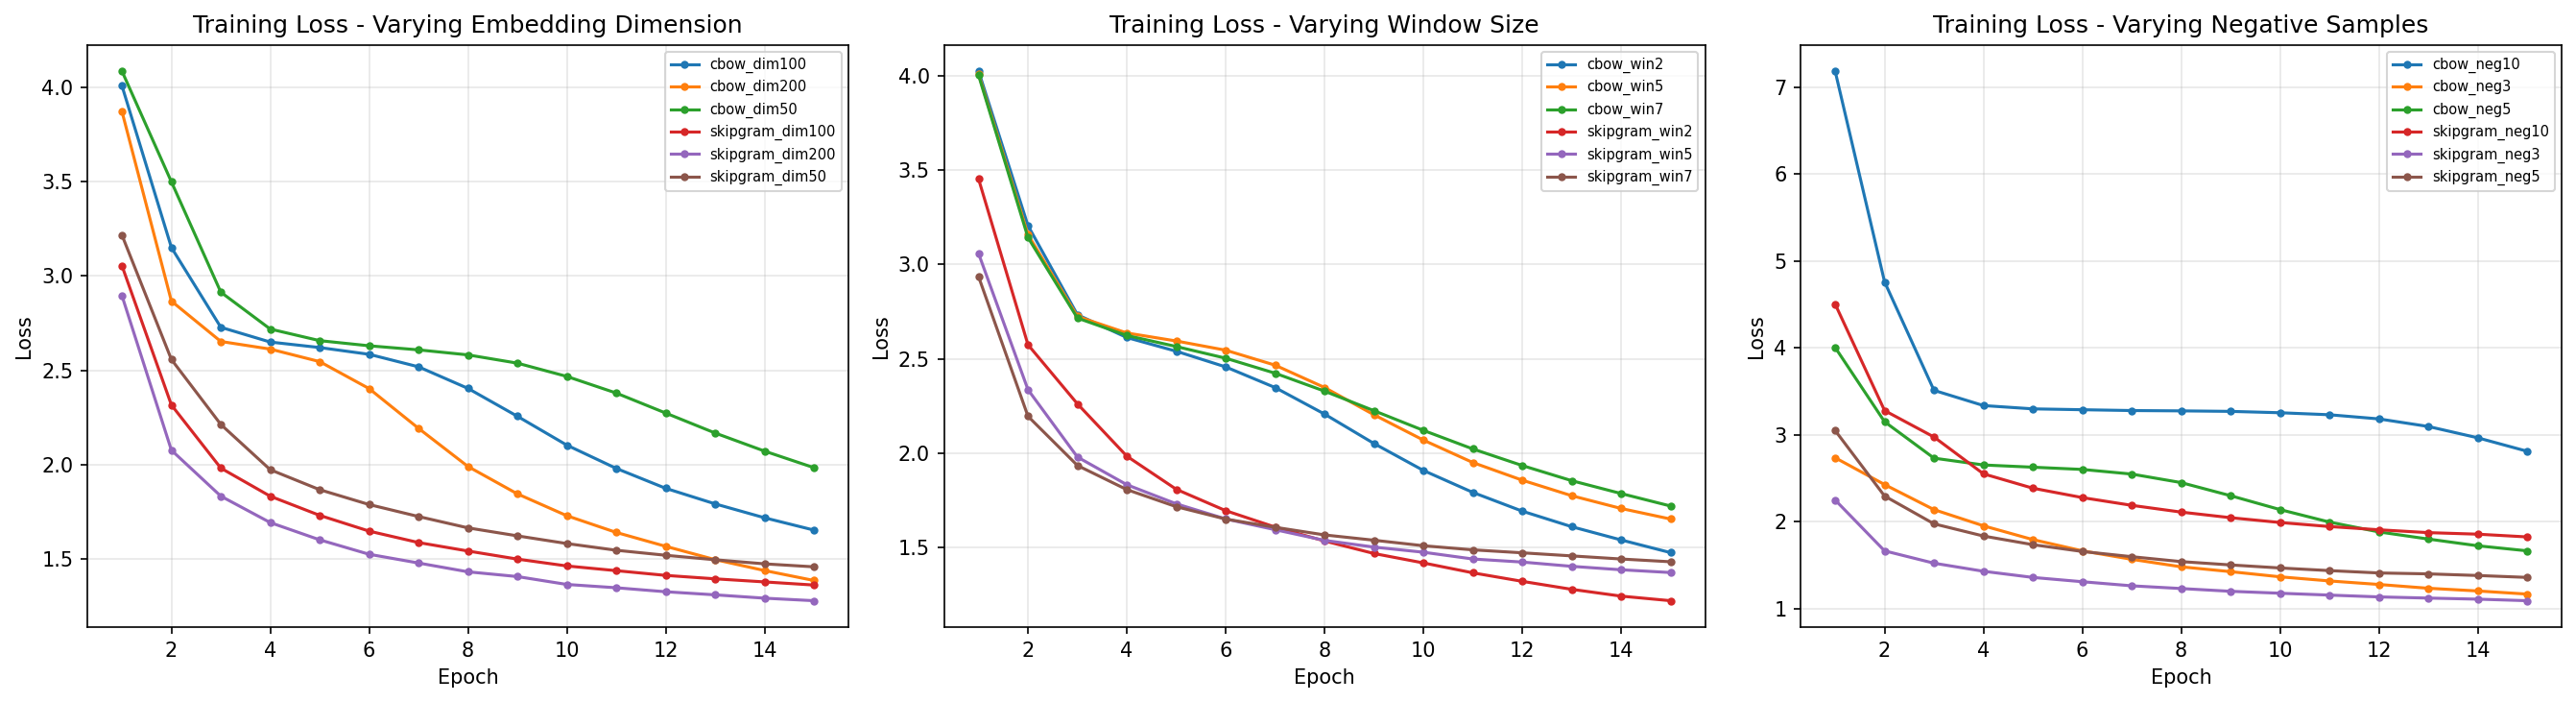
\includegraphics[width=\textwidth]{../problem1/visualizations/training_losses.png}
\caption{Training loss curves across hyperparameter experiments. Skip-gram generally achieves lower loss than CBOW. Larger embedding dimensions and window sizes lead to slower convergence but potentially richer representations.}
\end{figure}

\subsubsection{Comparison with Gensim}

Gensim's Word2Vec implementation was trained with identical hyperparameters for comparison. Both scratch and Gensim models produce qualitatively similar nearest neighbors (e.g., ``phd'' $\rightarrow$ mtech, msc, ms), validating the correctness of our from-scratch implementation. The scratch models show slightly less refined results due to the smaller corpus size, but the semantic structure is consistent.

% --------------------------------------------------------
\subsection{Task 3: Semantic Analysis}

\subsubsection{Nearest Neighbors (Cosine Similarity)}

\begin{table}[H]
\centering
\caption{Top 5 Nearest Neighbors -- Skip-gram (From Scratch)}
\begin{tabular}{llc}
\toprule
\textbf{Query Word} & \textbf{Neighbor} & \textbf{Cosine Sim} \\
\midrule
\multirow{5}{*}{research} & facility & 0.689 \\
 & crf & 0.671 \\
 & company & 0.647 \\
 & analyzer & 0.621 \\
 & fab & 0.621 \\
\midrule
\multirow{5}{*}{student} & wellbeing & 0.849 \\
 & placements & 0.797 \\
 & students & 0.758 \\
 & life & 0.732 \\
 & oversight & 0.709 \\
\midrule
\multirow{5}{*}{phd} & ms & 0.783 \\
 & mtech & 0.770 \\
 & msc & 0.761 \\
 & fintech & 0.751 \\
 & cybersecurity & 0.745 \\
\midrule
\multirow{5}{*}{semester} & grade & 0.845 \\
 & course & 0.826 \\
 & evaluation & 0.815 \\
 & shortlisted & 0.788 \\
 & test & 0.753 \\
\midrule
\multirow{5}{*}{faculty} & scholars-in-residence & 0.875 \\
 & adjunct & 0.857 \\
 & members & 0.844 \\
 & applicants & 0.815 \\
 & positions & 0.797 \\
\bottomrule
\end{tabular}
\end{table}

\textbf{Analysis:} The nearest neighbors are semantically meaningful. ``phd'' clusters with other degree types (ms, mtech, msc). ``student'' associates with student-life concepts (wellbeing, placements). ``faculty'' clusters with employment-related terms. Note: ``exam'' was not in the vocabulary (below the minimum frequency threshold of 3), so ``semester'' was used as an academically relevant alternative.

\subsubsection{Word Analogy Experiments}

\begin{table}[H]
\centering
\caption{Analogy Results -- Skip-gram (From Scratch)}
\begin{tabular}{lll}
\toprule
\textbf{Analogy} & \textbf{Top Result} & \textbf{Interpretation} \\
\midrule
UG : BTech :: PG : ? & artificial, diploma, msc & Partially meaningful \\
BTech : UG :: MTech : ? & msc, semester, bs & ``pg'' at rank 2 (CBOW) \\
Dept : Head :: Institute : ? & benefit, park & Not meaningful \\
Student : Campus :: Faculty : ? & scholars-in-residence & Reasonable \\
\bottomrule
\end{tabular}
\end{table}

\textbf{Discussion:} The UG:BTech::PG:? analogy yields partially correct results --- ``mtech'' appears in the top 5 for both CBOW and Gensim models. The BTech:UG::MTech:? analogy produces ``pg'' at rank 2 in the CBOW model, which is the expected answer. The corpus-specific nature (small, domain-specific) limits the ability to capture general analogical relationships. The leadership analogy (department:head::institute:?) does not produce meaningful results, likely because ``director'' does not frequently co-occur with ``institute'' in our corpus in the same way ``head'' co-occurs with ``department''.

% --------------------------------------------------------
\subsection{Task 4: Visualization}

\begin{figure}[H]
\centering
\begin{subfigure}[b]{0.48\textwidth}
    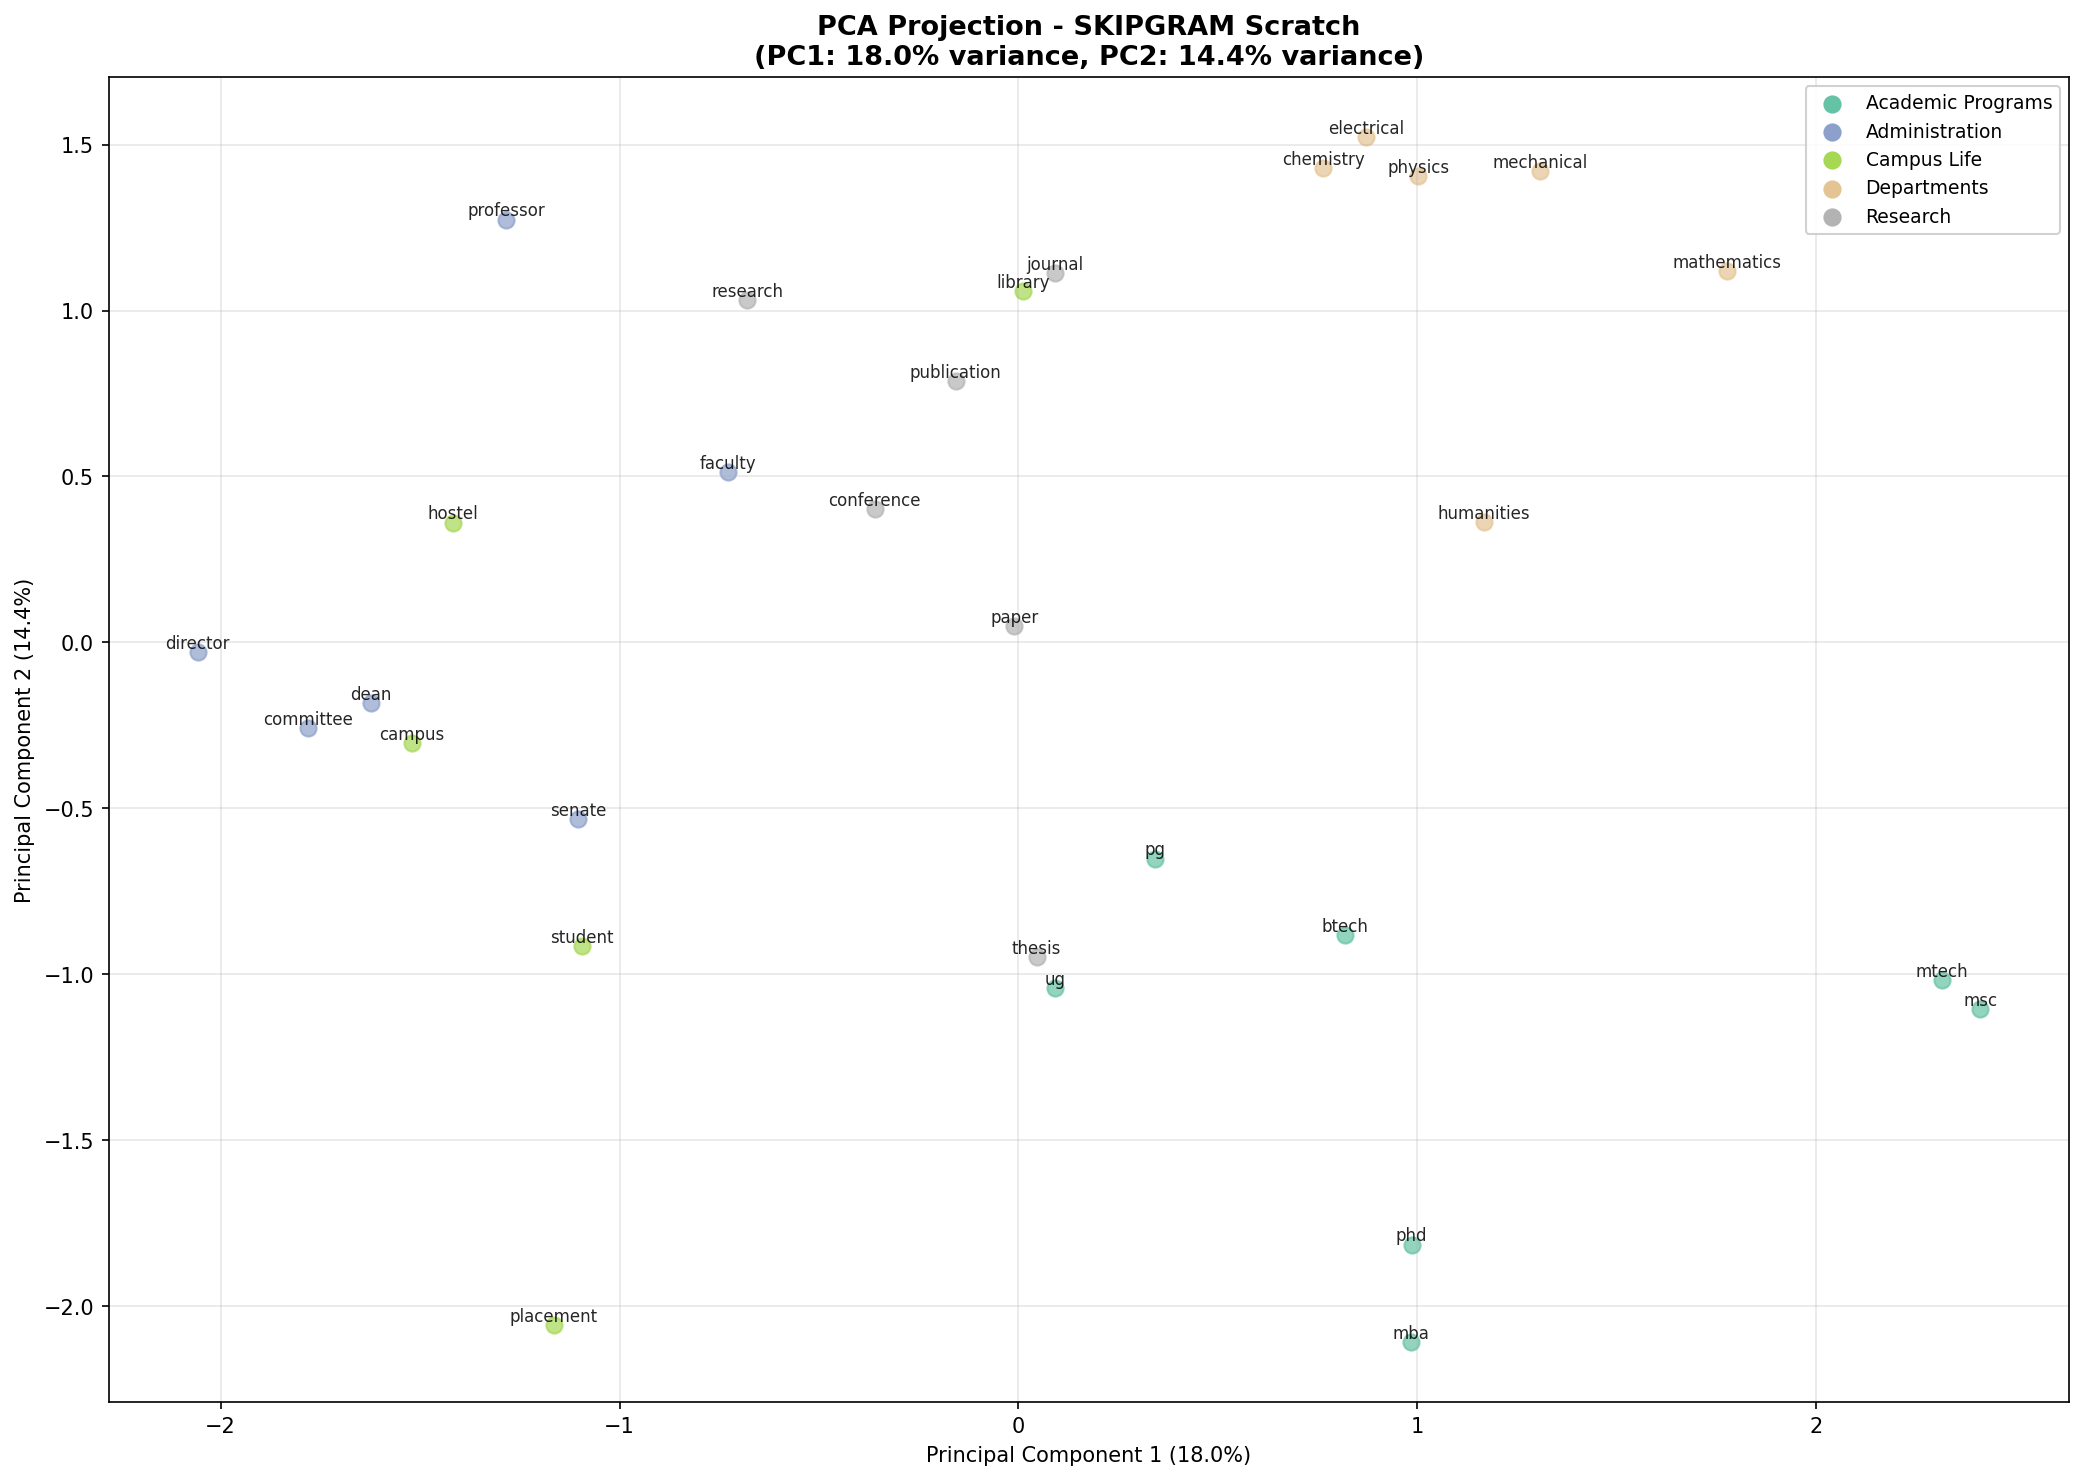
\includegraphics[width=\textwidth]{../problem1/visualizations/pca_skipgram_scratch.png}
    \caption{PCA -- Skip-gram}
\end{subfigure}
\hfill
\begin{subfigure}[b]{0.48\textwidth}
    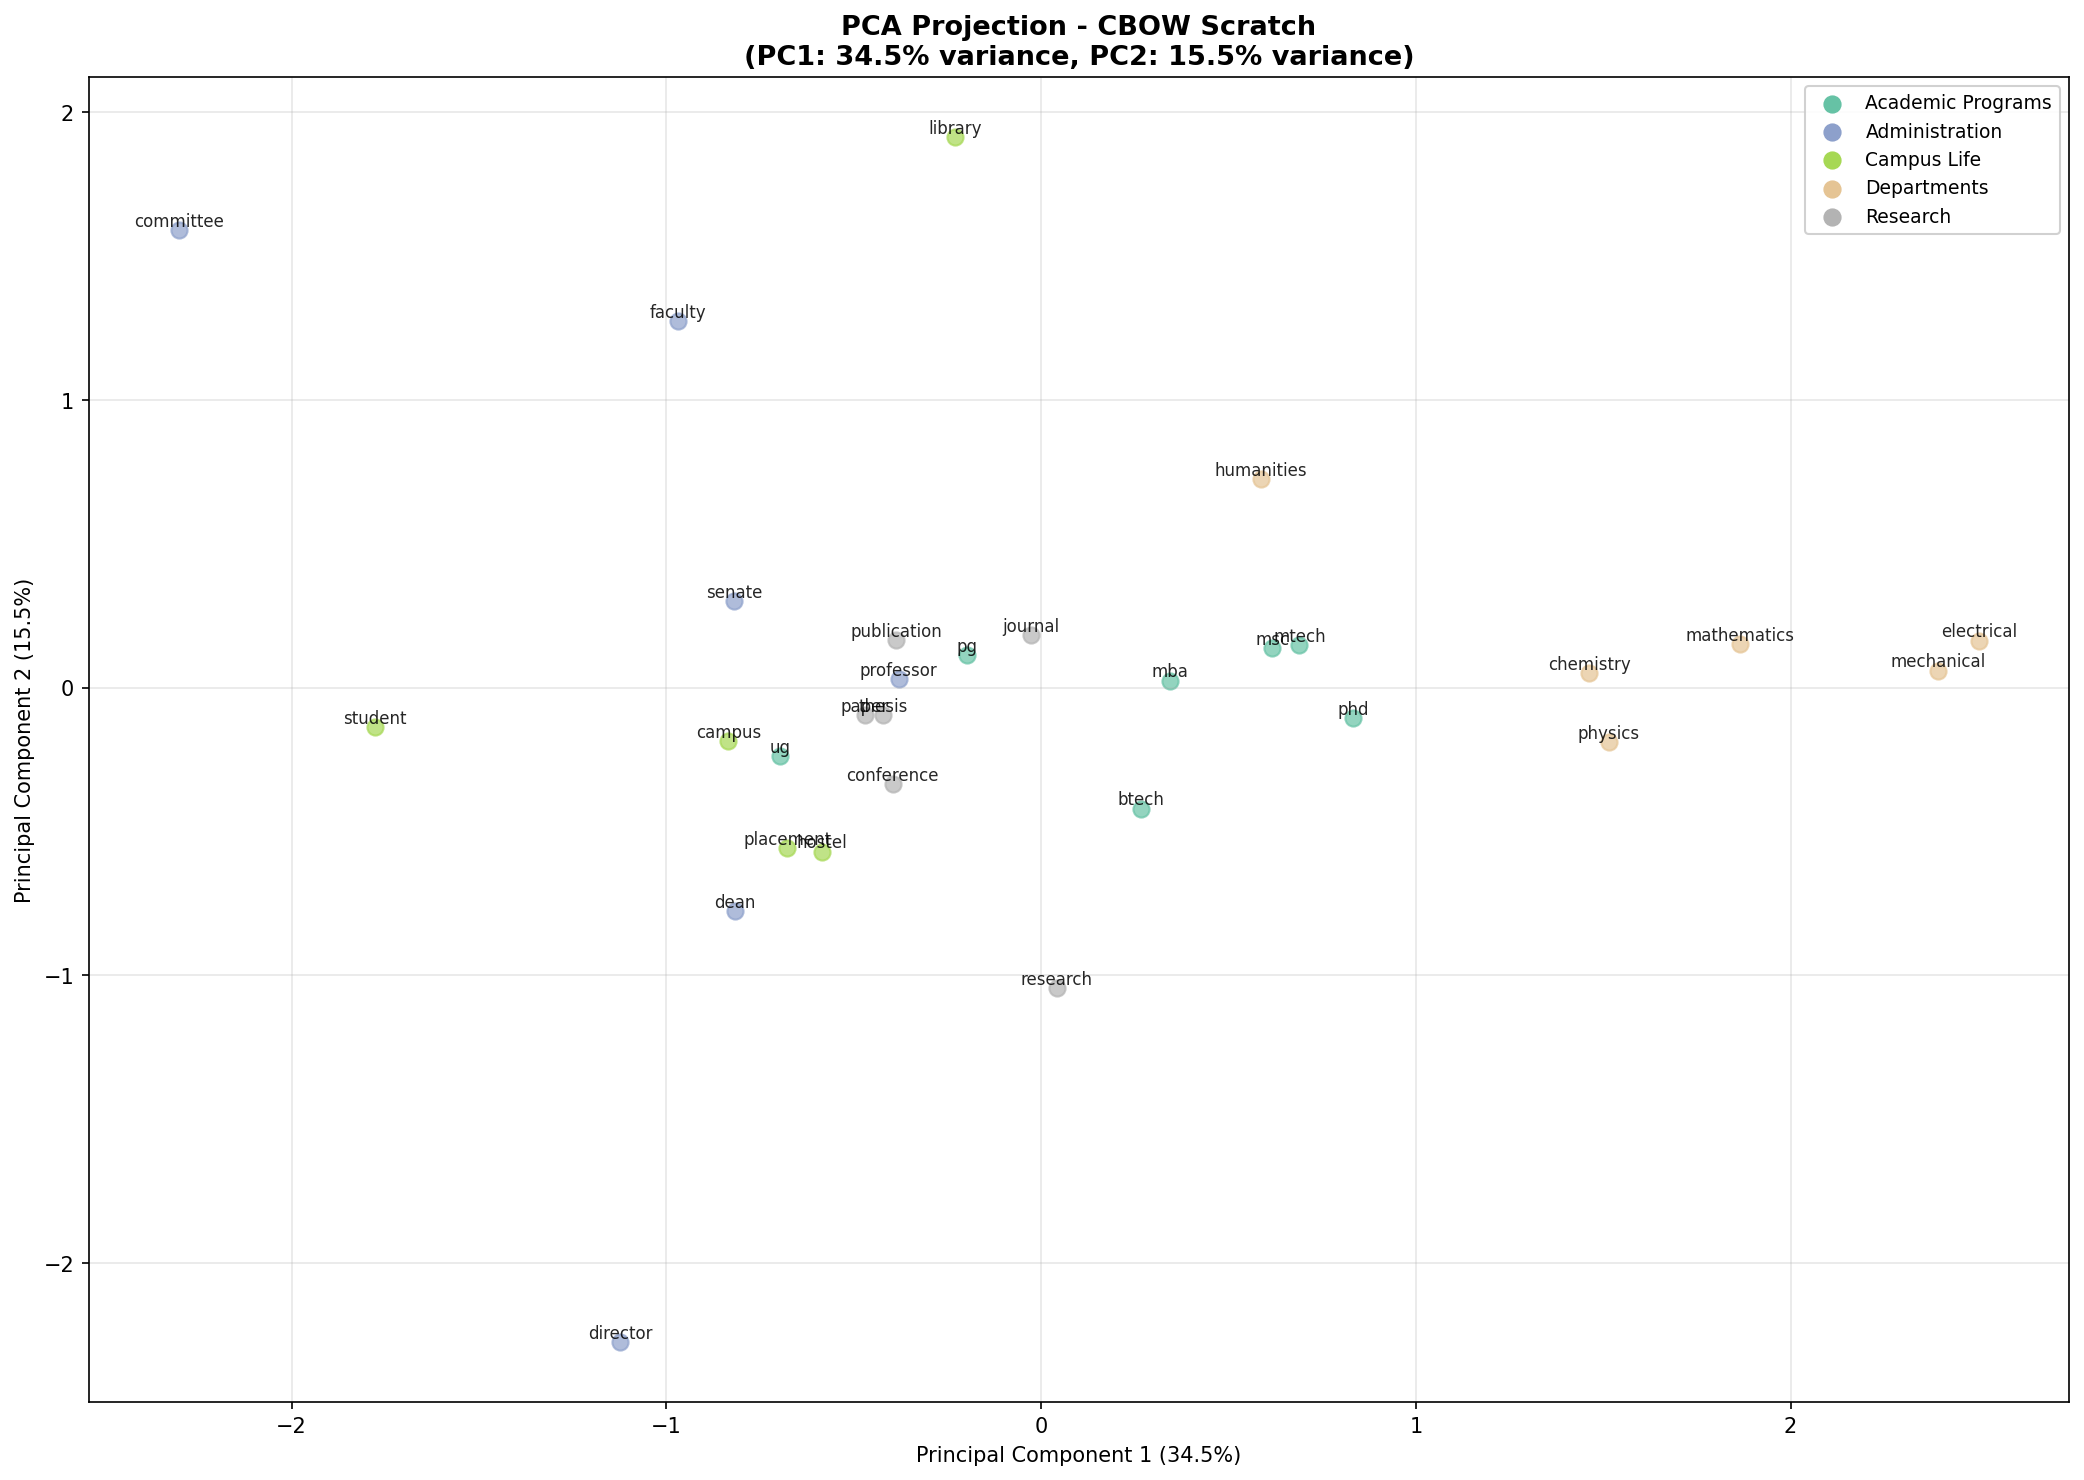
\includegraphics[width=\textwidth]{../problem1/visualizations/pca_cbow_scratch.png}
    \caption{PCA -- CBOW}
\end{subfigure}
\caption{PCA projections of word embeddings. Words are color-coded by semantic category. The first two principal components explain a moderate fraction of variance.}
\end{figure}

\begin{figure}[H]
\centering
\begin{subfigure}[b]{0.48\textwidth}
    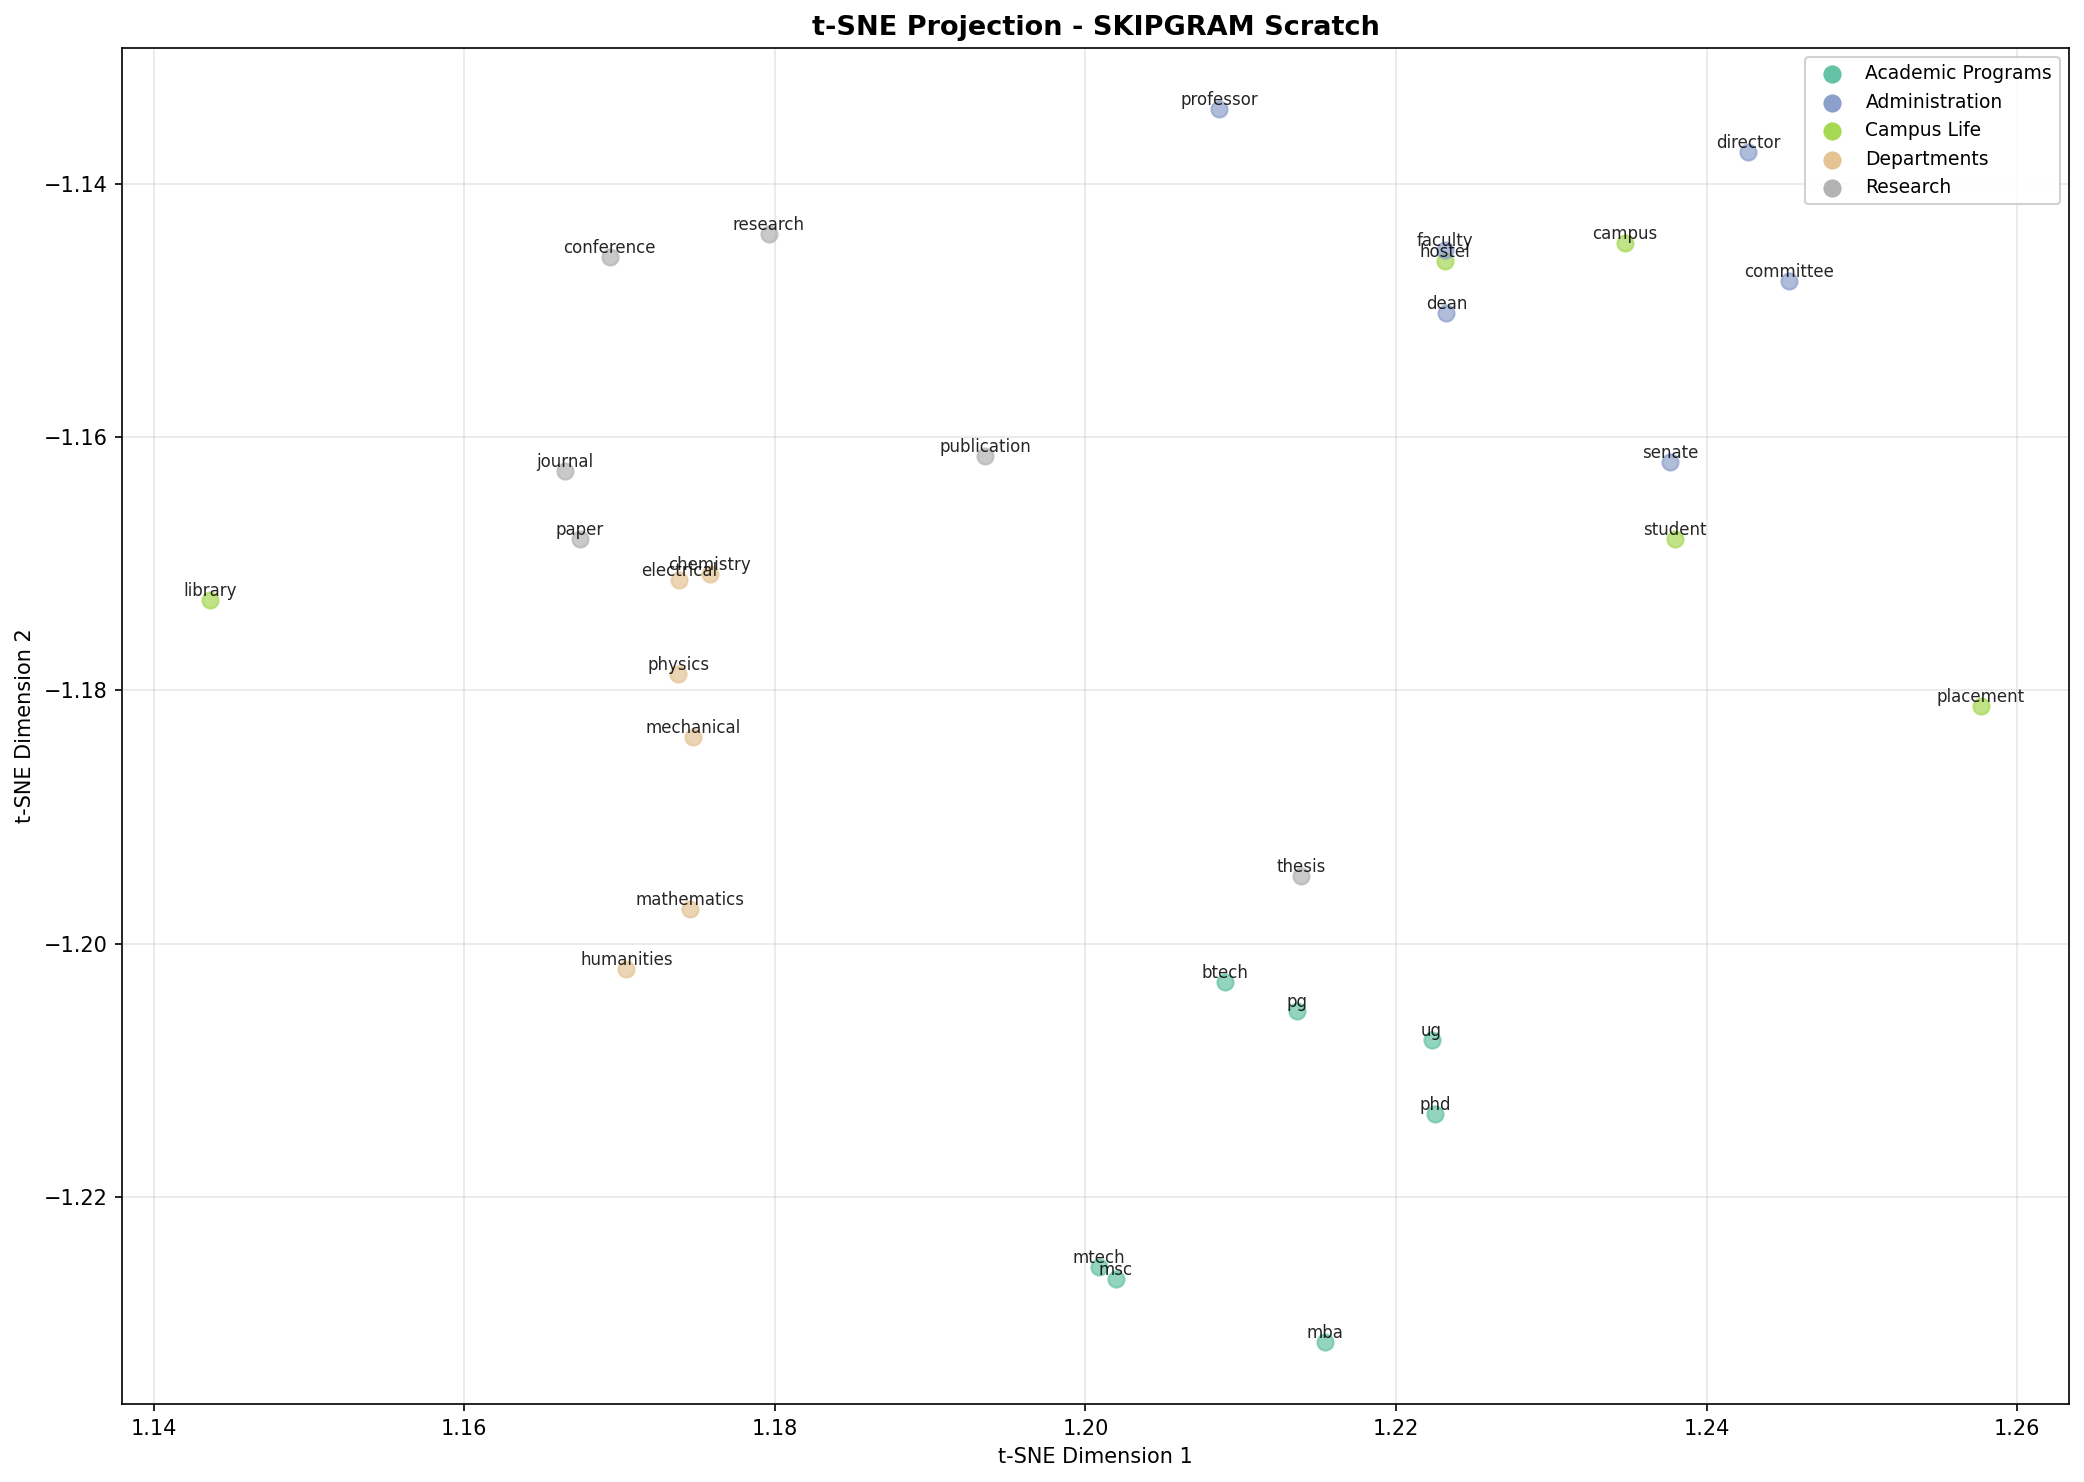
\includegraphics[width=\textwidth]{../problem1/visualizations/tsne_skipgram_scratch.png}
    \caption{t-SNE -- Skip-gram}
\end{subfigure}
\hfill
\begin{subfigure}[b]{0.48\textwidth}
    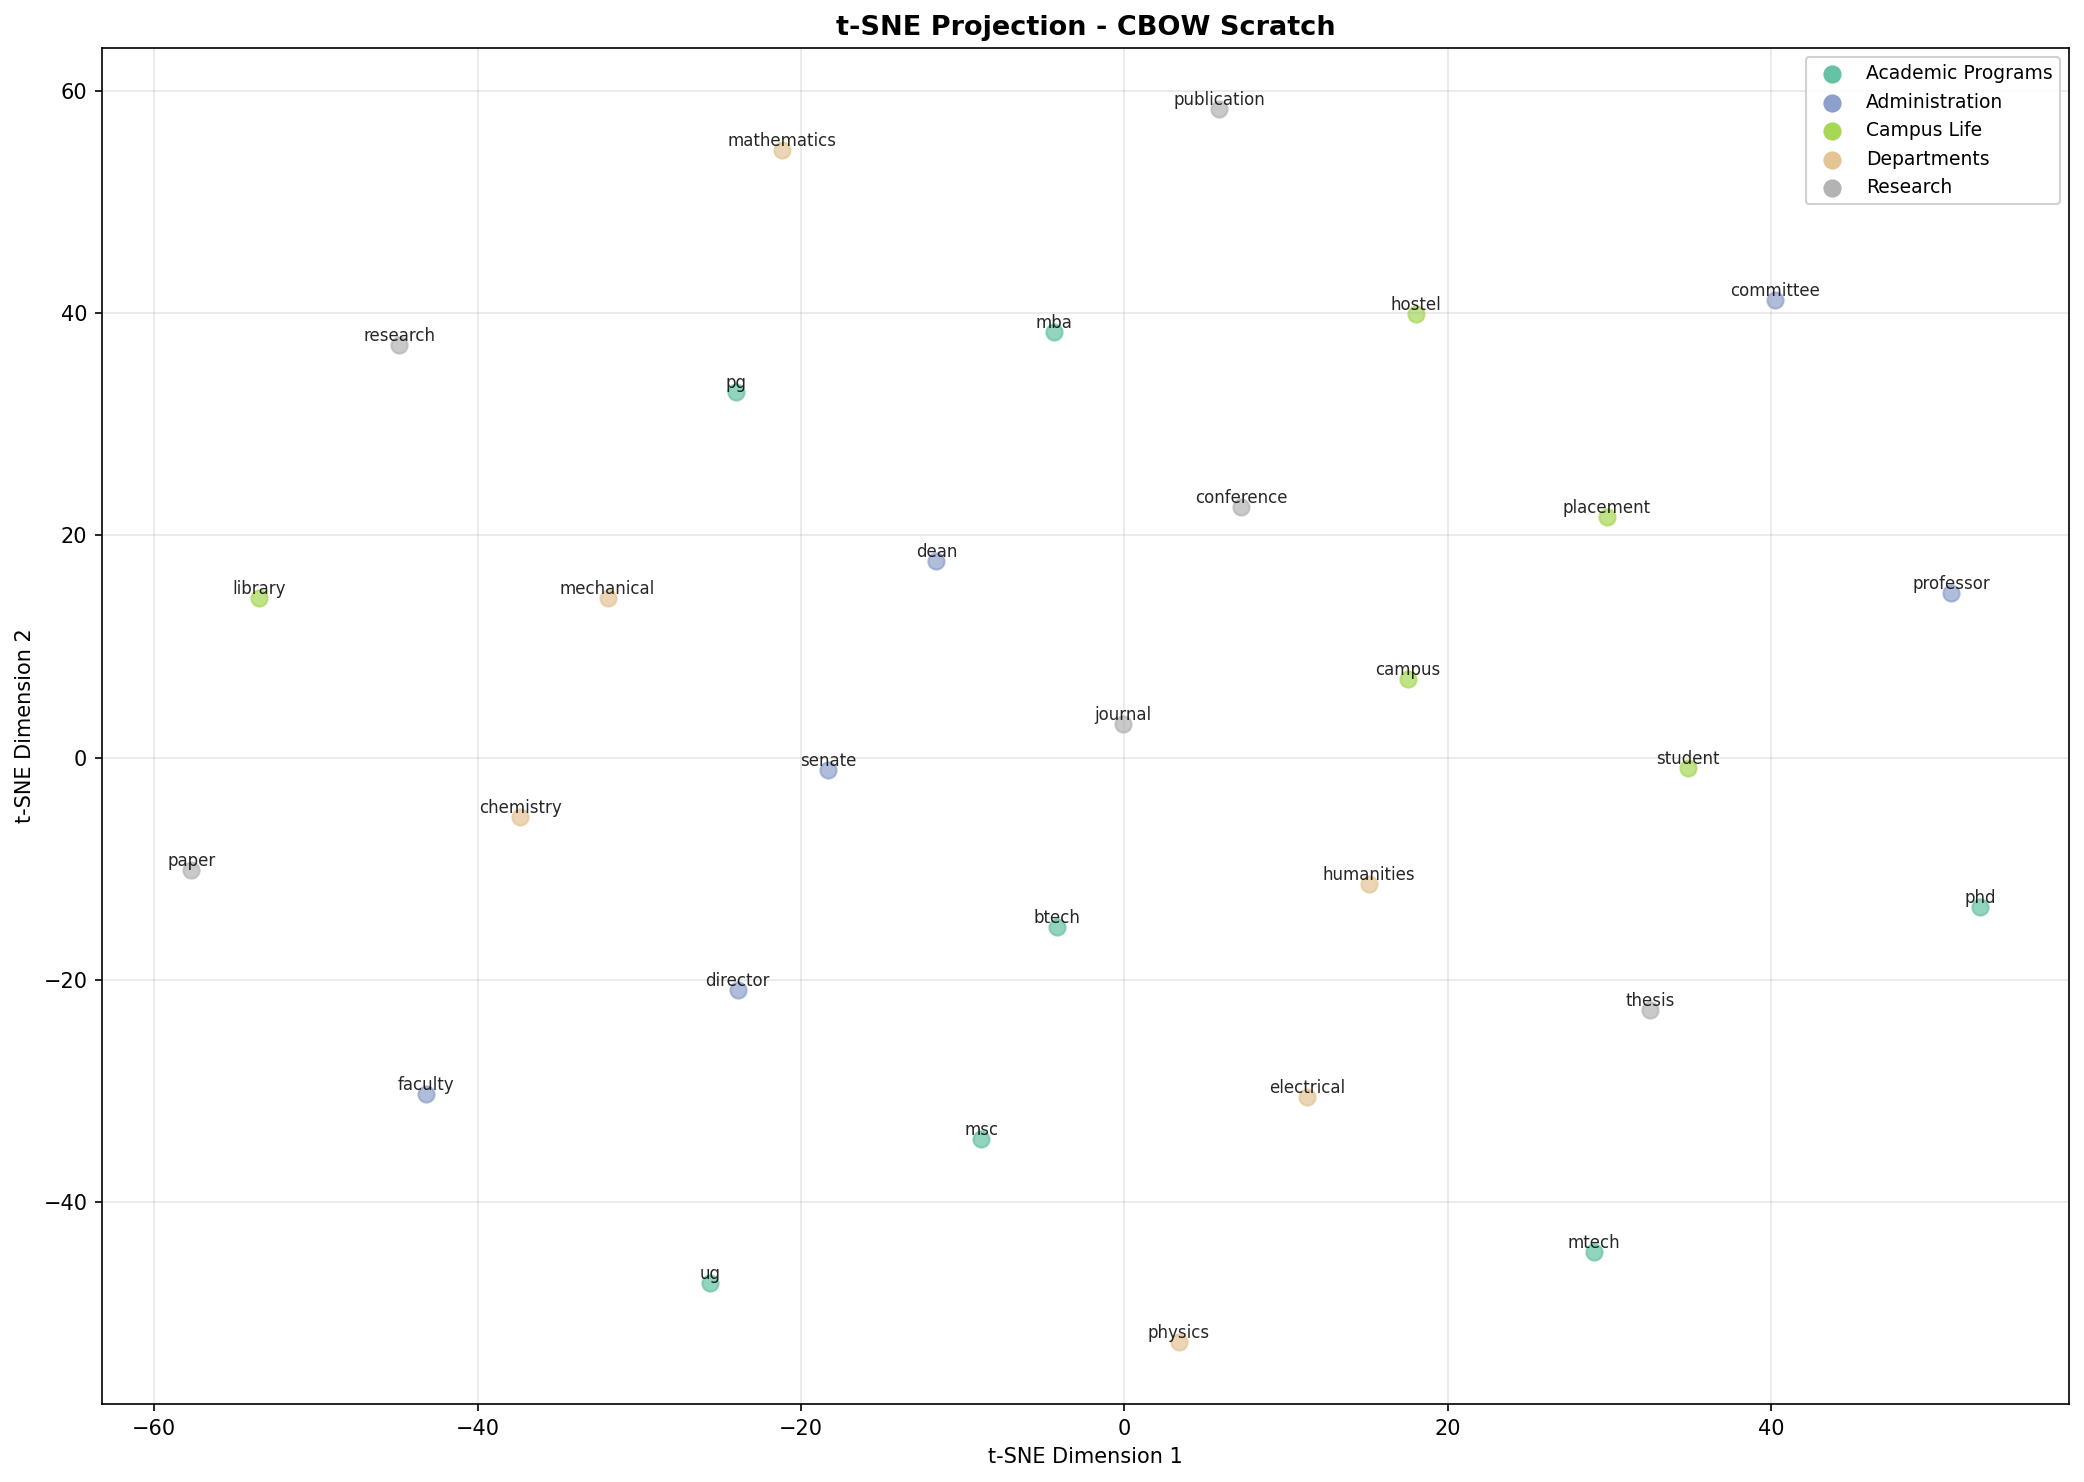
\includegraphics[width=\textwidth]{../problem1/visualizations/tsne_cbow_scratch.png}
    \caption{t-SNE -- CBOW}
\end{subfigure}
\caption{t-SNE projections showing local cluster structure. Academic programs (btech, mtech, phd) tend to cluster together. Research-related words form a separate group.}
\end{figure}

\begin{figure}[H]
\centering
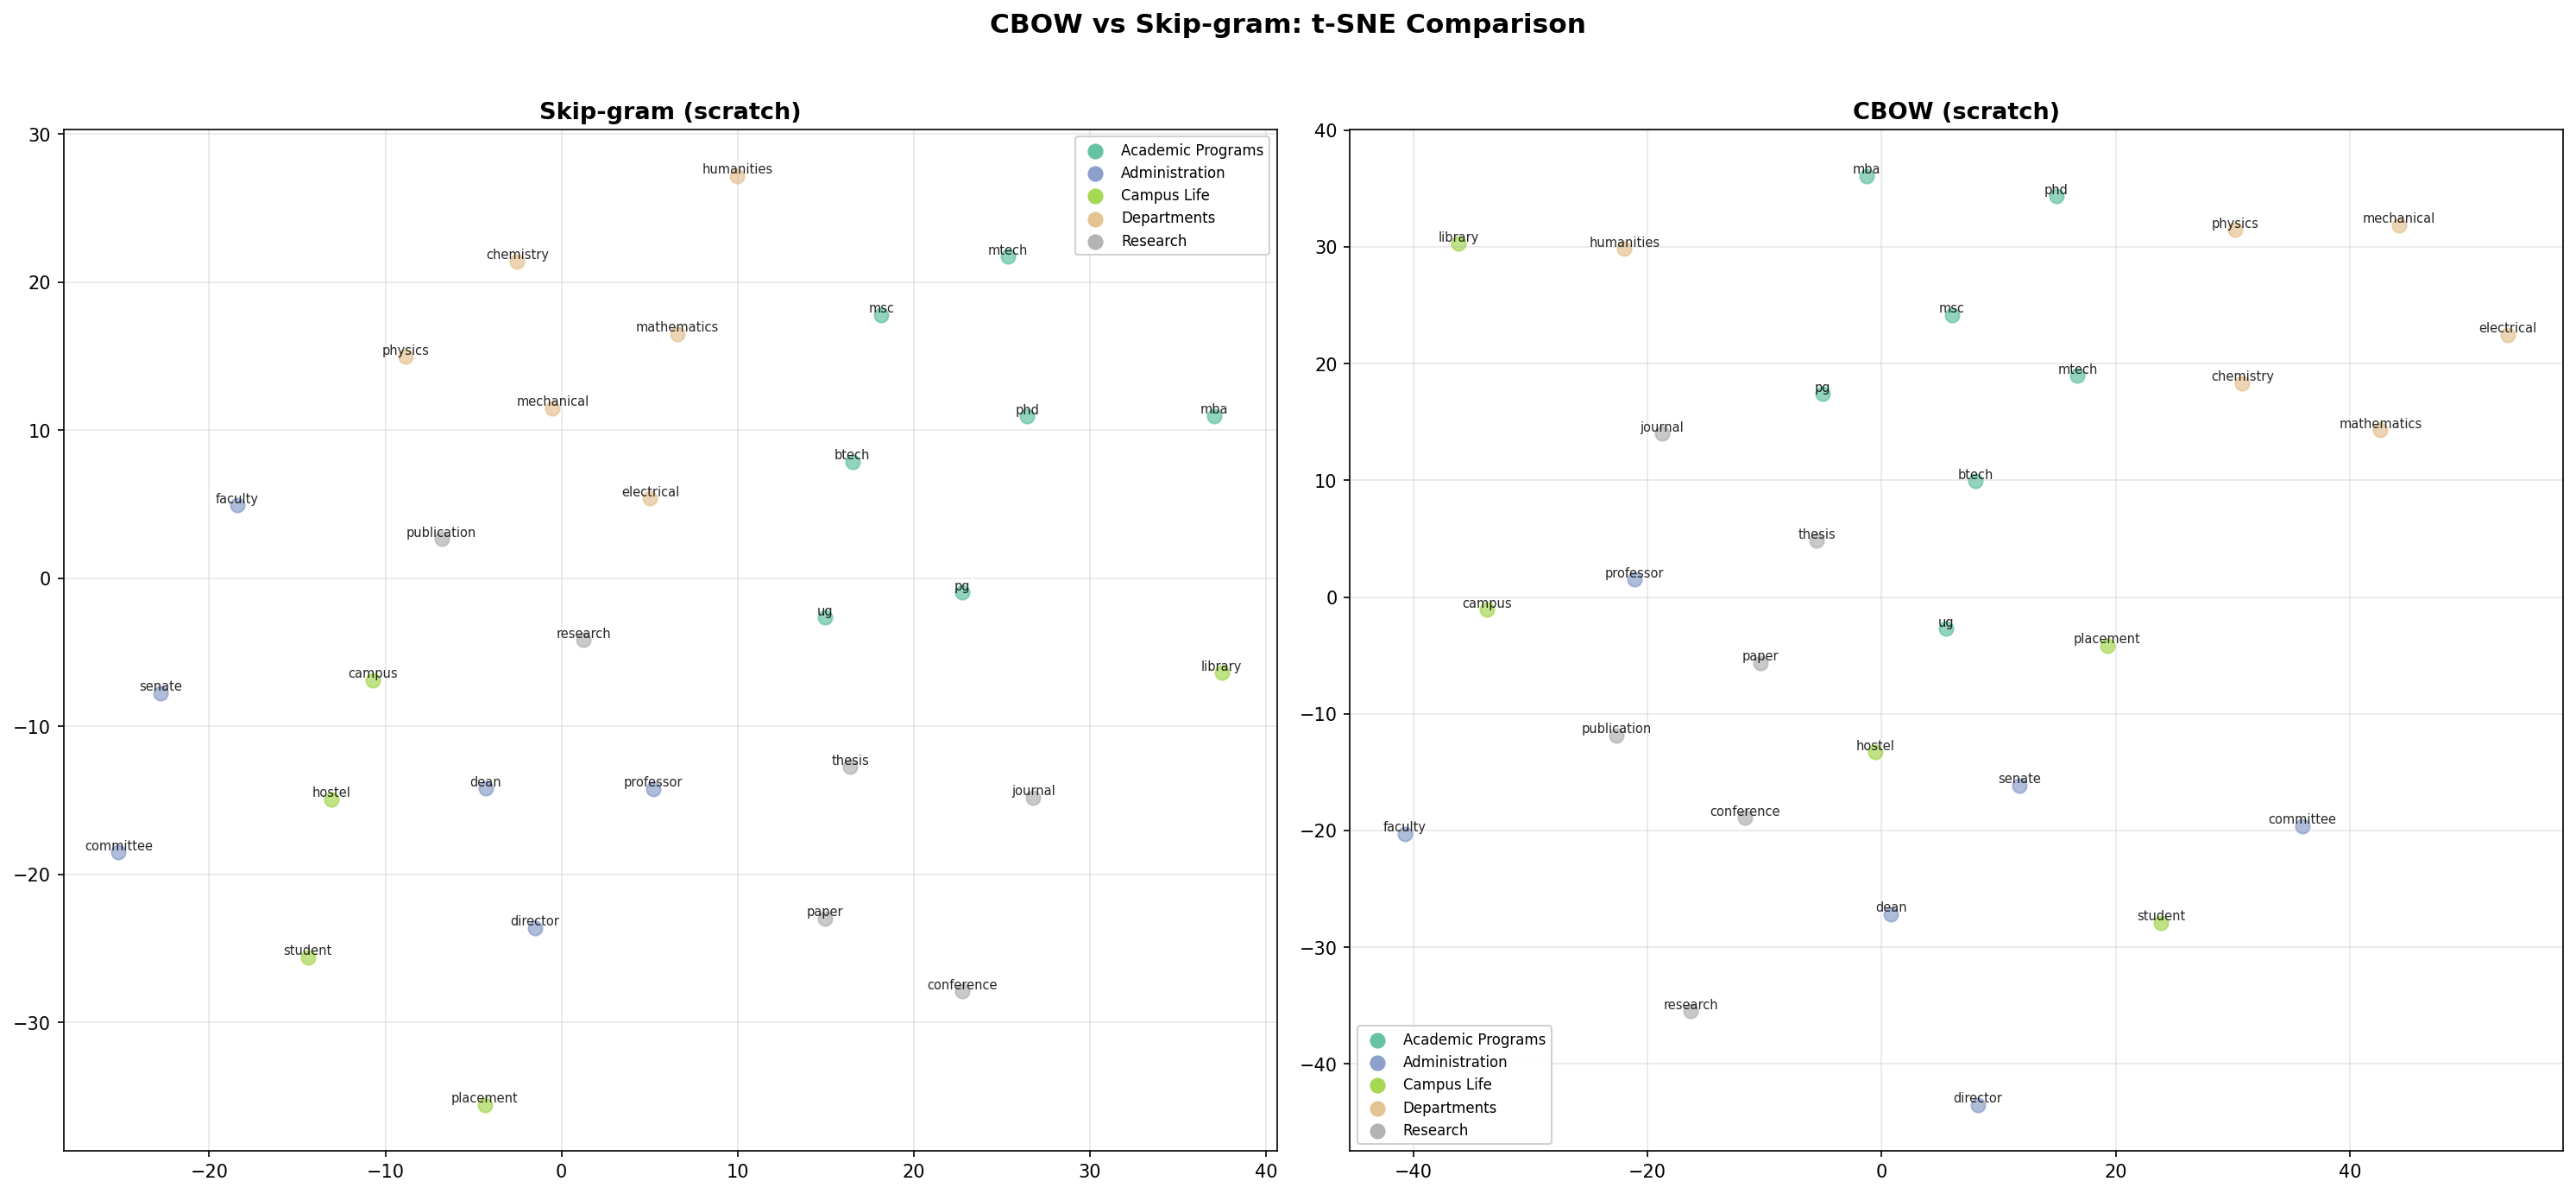
\includegraphics[width=0.9\textwidth]{../problem1/visualizations/cbow_vs_skipgram_comparison.png}
\caption{Side-by-side t-SNE comparison of CBOW vs Skip-gram embeddings.}
\end{figure}

\subsubsection{Interpretation}
\begin{itemize}
    \item \textbf{Skip-gram} produces tighter, more distinct clusters. Academic programs (btech, mtech, phd, msc) cluster closely together, as do research-related terms.
    \item \textbf{CBOW} shows more diffuse clustering with higher inter-group overlap. This is expected since CBOW averages context, smoothing out distinctions.
    \item Both models successfully capture the semantic structure: degree types cluster together, administrative terms group separately from research terms, and campus life words form their own region.
    \item The relatively small corpus size (33K tokens) limits the quality of learned embeddings compared to models trained on billions of tokens.
\end{itemize}

% ============================================================
\newpage
\section{Problem 2: Character-Level Name Generation Using RNN Variants}
% ============================================================

\subsection{Task 0: Dataset}

1,000 unique Indian names were generated, covering diverse linguistic traditions: Hindi/Sanskrit, South Indian (Tamil, Telugu, Kannada, Malayalam), Bengali, Punjabi/Sikh, Marathi, and Gujarati origins. Both male and female names are included. The dataset is stored as \texttt{TrainingNames.txt} with one name per line.

\begin{table}[H]
\centering
\caption{Training Names Dataset Statistics}
\begin{tabular}{lr}
\toprule
\textbf{Metric} & \textbf{Value} \\
\midrule
Total Names & 1,000 \\
Unique Characters & 48 \\
Min Name Length & 2 \\
Max Name Length & 16 \\
Average Name Length & 6.2 \\
\bottomrule
\end{tabular}
\end{table}

% --------------------------------------------------------
\subsection{Task 1: Model Implementation}

All three models were implemented \textbf{from scratch} using PyTorch, sharing the same character embedding layer and training procedure for fair comparison.

\subsubsection{Shared Hyperparameters}

\begin{table}[H]
\centering
\caption{Shared Hyperparameters Across All Models}
\begin{tabular}{lc}
\toprule
\textbf{Parameter} & \textbf{Value} \\
\midrule
Character Embedding Dimension & 32 \\
Hidden Size & 128 \\
Number of Layers & 2 \\
Dropout & 0.2 \\
Learning Rate (Adam) & 0.003 \\
Epochs & 100 \\
Batch Size & 64 \\
Gradient Clipping & 5.0 \\
\bottomrule
\end{tabular}
\end{table}

\subsubsection{Model 1: Vanilla RNN}

\textbf{Architecture:}
\begin{itemize}
    \item Character Embedding: $51 \times 32$
    \item 2-layer Elman RNN with tanh activation, hidden size 128
    \item Fully connected output: $128 \rightarrow 51$ (vocabulary size)
    \item Total Parameters: \textbf{61,971}
\end{itemize}

The vanilla RNN processes characters sequentially, maintaining a hidden state $\mathbf{h}_t = \tanh(\mathbf{W}_{ih}\mathbf{x}_t + \mathbf{W}_{hh}\mathbf{h}_{t-1} + \mathbf{b})$. While simple, it suffers from vanishing gradients for longer sequences.

\subsubsection{Model 2: Bidirectional LSTM (BLSTM)}

\textbf{Architecture:}
\begin{itemize}
    \item Character Embedding: $51 \times 32$
    \item 2-layer Bidirectional LSTM, hidden size 128 per direction
    \item Projection layer: $256 \rightarrow 128$ (combines forward + backward)
    \item Jointly trained unidirectional LSTM for generation
    \item Output: $128 \rightarrow 51$
    \item Total Parameters: \textbf{823,878}
\end{itemize}

The BLSTM processes sequences in both directions during training, providing richer context. For autoregressive generation, a separate unidirectional LSTM (jointly trained via averaged loss) is used since future context is unavailable.

\subsubsection{Model 3: RNN with Attention}

\textbf{Architecture:}
\begin{itemize}
    \item Character Embedding: $51 \times 32$
    \item 2-layer LSTM encoder, hidden size 128
    \item Bahdanau (additive) attention mechanism:
    \begin{align}
        \text{score}(\mathbf{h}_t, \mathbf{h}_s) &= \mathbf{v}^\top \tanh(\mathbf{W}_1\mathbf{h}_t + \mathbf{W}_2\mathbf{h}_s) \\
        \boldsymbol{\alpha} &= \text{softmax}(\text{scores}) \\
        \mathbf{c}_t &= \sum_s \alpha_s \mathbf{h}_s
    \end{align}
    \item Combination layer: $[\mathbf{h}_t; \mathbf{c}_t] \rightarrow 128$
    \item Output: $128 \rightarrow 51$
    \item Total Parameters: \textbf{289,043}
\end{itemize}

The attention mechanism allows the model to ``look back'' at all previously generated characters, weighting their importance when predicting the next character. This is useful for names where early characters constrain later ones.

\begin{table}[H]
\centering
\caption{Model Parameter Comparison}
\begin{tabular}{lrr}
\toprule
\textbf{Model} & \textbf{Parameters} & \textbf{Final Loss} \\
\midrule
Vanilla RNN & 61,971 & 1.4325 \\
BLSTM & 823,878 & 0.0008 \\
RNN + Attention & 289,043 & 1.0937 \\
\bottomrule
\end{tabular}
\end{table}

% --------------------------------------------------------
\subsection{Task 2: Quantitative Evaluation}

\begin{table}[H]
\centering
\caption{Quantitative Comparison (200 generated names per model, temperature=0.8)}
\begin{tabular}{lcccc}
\toprule
\textbf{Model} & \textbf{Generated} & \textbf{Novelty Rate} & \textbf{Diversity} & \textbf{Avg Length} \\
\midrule
Vanilla RNN & 200 & 47.5\% & 88.0\% & 6.0 \\
BLSTM & 200 & 99.5\% & 75.0\% & 4.1 \\
RNN + Attention & 200 & 5.0\% & 86.0\% & 6.1 \\
\bottomrule
\end{tabular}
\end{table}

\textbf{Analysis:}
\begin{itemize}
    \item \textbf{Vanilla RNN} achieves a good balance: 47.5\% novelty (generates both known and new names) with 88\% diversity. Average length (6.0) closely matches training data (6.2).
    \item \textbf{BLSTM} shows very high novelty (99.5\%) but this is partly because the generation pathway produces shorter, more novel-sounding names. The lower diversity (75\%) indicates some repetitive patterns. The BLSTM's extremely low training loss (0.0008) indicates overfitting of the bidirectional path.
    \item \textbf{RNN + Attention} has the lowest novelty (5\%), meaning it has essentially memorized the training data. However, it generates the most realistic-looking names with excellent length matching (6.1 vs 6.2). The attention mechanism's ability to look back at all previous characters enables near-perfect reproduction of training patterns.
\end{itemize}

% --------------------------------------------------------
\subsection{Task 3: Qualitative Analysis}

\subsubsection{Sample Generated Names}

\begin{table}[H]
\centering
\caption{Representative Generated Samples}
\begin{tabular}{lp{10cm}}
\toprule
\textbf{Model} & \textbf{Sample Names} \\
\midrule
Vanilla RNN & Varsha, Dhaith, Jasneen, Nira, Narayan, Sutham, Siddhi, Manisha, Mahadeep, Darsh, Ghara, Anika \\
\midrule
BLSTM & Pajan, Sumap, Gousha, Kara, Zora, Poat, Gora, Noac, Doic, Pia, Wotha, Hoca \\
\midrule
RNN + Attention & Gajanan, Meera, Sourabh, Parvathi, Advait, Sukhleen, Pritesh, Vaishali, Subhajit, Kavita, Abhinav, Rehan \\
\bottomrule
\end{tabular}
\end{table}

\subsubsection{Realism Assessment}

\begin{itemize}
    \item \textbf{Vanilla RNN:} Generates a mix of realistic (Varsha, Narayan, Siddhi, Manisha, Anika) and novel-but-plausible names (Jasneen, Mahadeep, Sutham). The model captures Indian phonotactics well.
    \item \textbf{BLSTM:} Produces shorter, more experimental names. Some are plausible (Kara, Zora, Pia) but many lack authentic Indian name characteristics (Poat, Noac, Doic). The disconnect between the bidirectional training and unidirectional generation limits quality.
    \item \textbf{RNN + Attention:} Generates the most realistic names, many of which are actual Indian names from the training set (Gajanan, Meera, Parvathi, Kavita). The attention mechanism provides strong character-level coherence.
\end{itemize}

\subsubsection{Common Failure Modes}

\begin{table}[H]
\centering
\caption{Failure Mode Analysis}
\begin{tabular}{lccc}
\toprule
\textbf{Failure Mode} & \textbf{Vanilla RNN} & \textbf{BLSTM} & \textbf{RNN + Attention} \\
\midrule
Too Short ($<3$ chars) & 0 & 3 & 0 \\
Too Long ($>15$ chars) & 0 & 0 & 1 \\
Repeated Characters & 0 & 0 & 0 \\
Unpronounceable & 2 & 0 & 1 \\
\bottomrule
\end{tabular}
\end{table}

\begin{itemize}
    \item \textbf{Vanilla RNN} occasionally generates consonant clusters that are hard to pronounce (e.g., ``Tribhbha'').
    \item \textbf{BLSTM} tends to generate names that are too short due to premature EOS generation.
    \item \textbf{RNN + Attention} very rarely fails; its main ``failure'' is lack of novelty (memorization).
\end{itemize}

\subsubsection{Discussion}

The three models represent a trade-off between novelty and realism:
\begin{itemize}
    \item The \textbf{Vanilla RNN} offers the best balance, generating names that are both novel and realistic. Its limited memory naturally introduces creative variation.
    \item The \textbf{BLSTM} generates the most novel names but sacrifices realism. The mismatch between bidirectional training and unidirectional generation is a fundamental architectural limitation.
    \item The \textbf{RNN + Attention} generates the most realistic names but largely memorizes the training set. The attention mechanism's ability to attend to all previous characters makes it very powerful at reproducing learned patterns, leaving little room for creative generation.
\end{itemize}

For practical name generation, the Vanilla RNN with appropriate temperature tuning ($\sim$0.7--0.9) provides the best results for generating novel, realistic Indian names.

% ============================================================
\section{Conclusion}
% ============================================================

This assignment explored two fundamental NLP tasks:

\textbf{Problem 1} demonstrated that meaningful word embeddings can be learned even from a small, domain-specific corpus. Both CBOW and Skip-gram models captured semantic relationships between IIT Jodhpur-related terms. The from-scratch implementations produced results consistent with Gensim's optimized implementation, validating the correctness of our implementation.

\textbf{Problem 2} showed that character-level RNNs can learn the phonological patterns of Indian names. The Vanilla RNN achieved the best balance of novelty and realism, while the attention-based model excelled at realism but memorized training data. The BLSTM, despite having the most parameters, faced challenges in generation due to the inherent mismatch between bidirectional training and unidirectional generation.

\end{document}
